\subsection{Magic 3D}
\label{Magic3D}

Shap-E involves training an encoder which "produces a latent representation of a 3D asset" \citep{junShapeE}. In a second step, a diffusion prior on the obtained latent representations is trained, conditioning it on images or text descriptions to capture additional information \citep{junShapeE}.

\begin{figure}[ht]
    \centering
      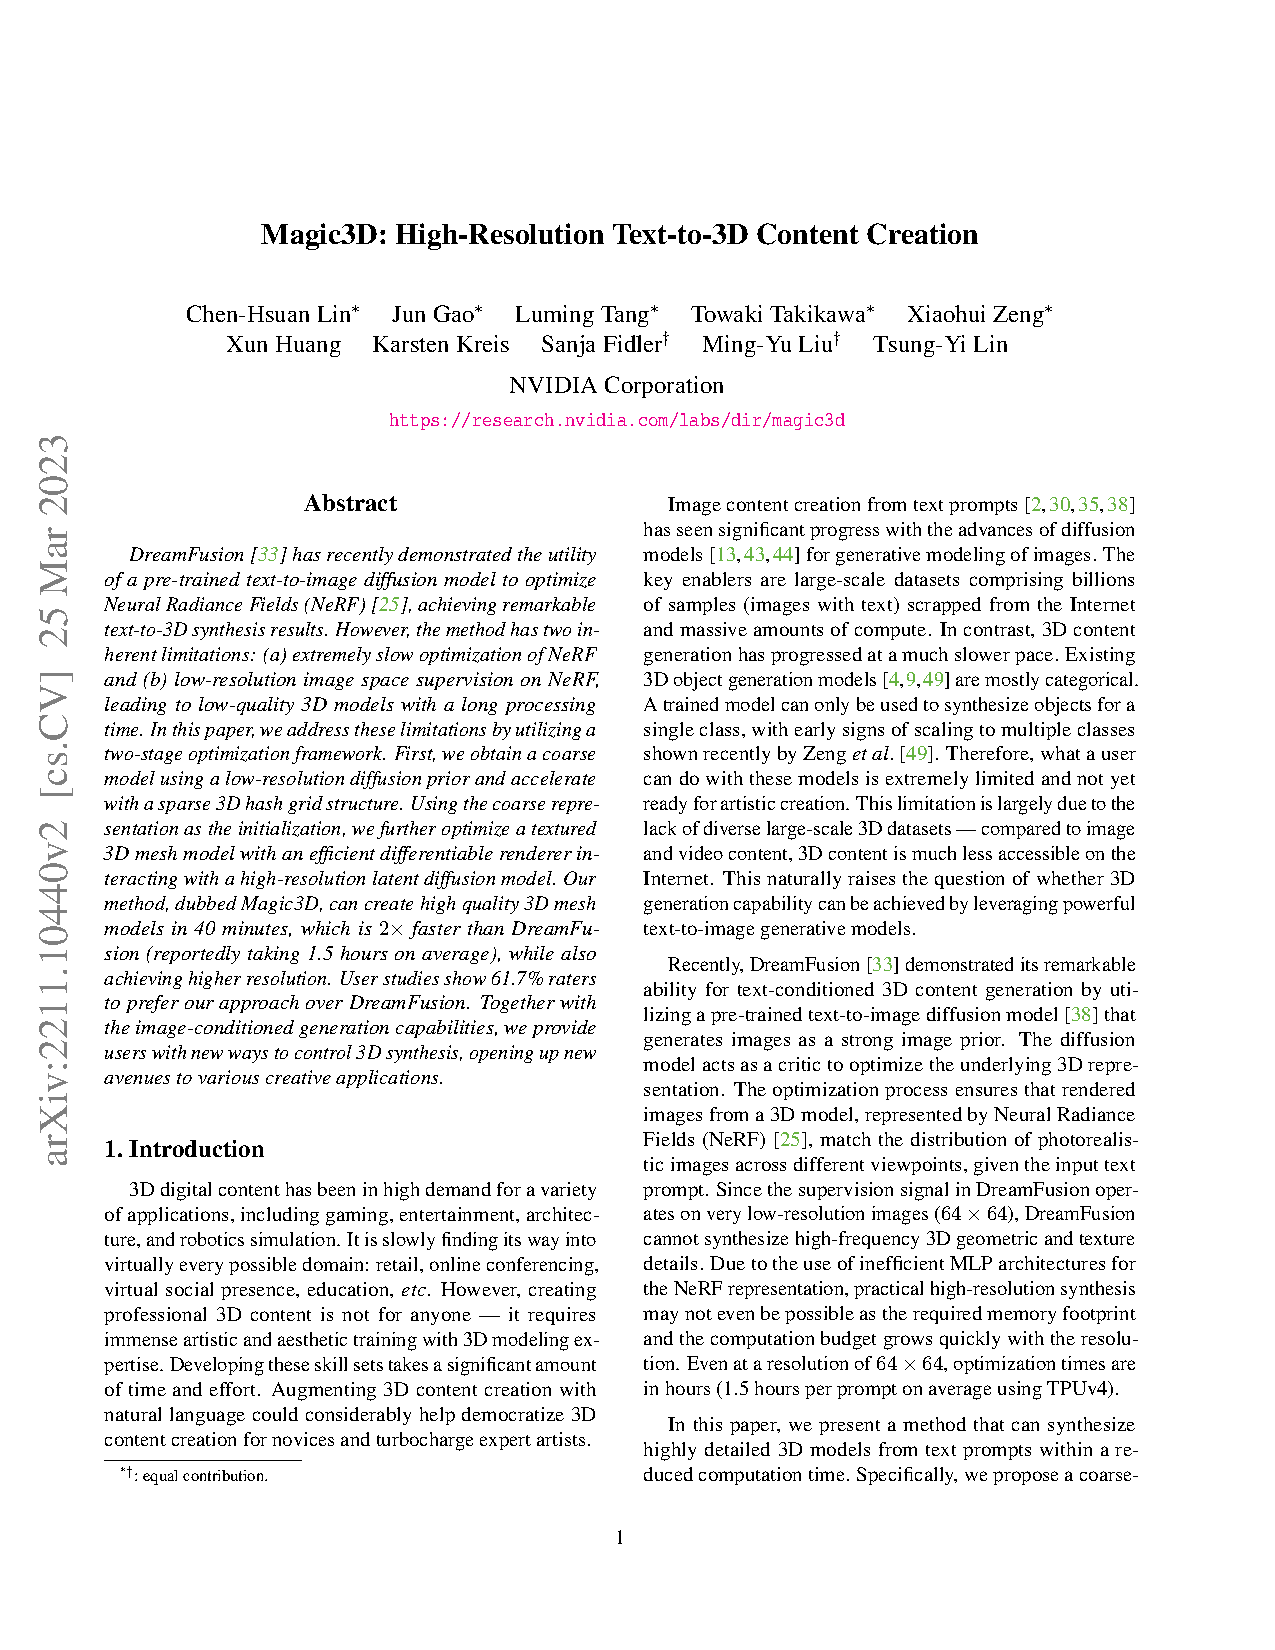
\includegraphics[width=1\columnwidth]{figures/Magic3D.png}
      \caption{Summatized functionality of Magic3D}\label{fig:figureMagic3D}
\end{figure}